\begin{figure}
    \centering
    \begin{subfigure}[t]{0.45\textwidth}
        \centering
        \begin{tikzpicture}[actor/.style={draw, minimum width=1.5cm}]
            \node[actor] (a) at (-1,0) {Alice};
            \node[actor] (b) at (1,0) {Bob};
            \node[actor] (kgc) at (0,1.5) {KGC};
        
            \node[above, align=center] at (kgc.north) {$\{PK, MK\}:=\text{Setup}()$};

            \node[below, align=center] at (a.south) {$\{m, \omega\}$\\};
            \node[below, align=center] at (b.south) {$\{\}$};

            % \draw[->] (a) edge node[left] {\{$S_A$\}} (kgc);
            % \draw[->] (b) edge node [right] {\{$S_B$\}} (kgc);
            % \draw[->] (a) edge pic [left=0.5cm, scale=0.05] {key} node [left=.5cm] {k} (kgc);
            \draw[-] (b) edge pic [right=0.5cm, scale=0.5, blue] {tree} node [right=.75cm, blue] {$S_B$} (kgc);
            % TODO fix arrows
            \draw (a) edge pic [left=0.5cm, scale=0.5, olive] {tree} node [left=.75cm, olive] {$S_A$} (kgc);
            % \draw[->] (b) edge node [right] {\{$S_B$\}} (kgc);

        \end{tikzpicture}
        \caption{The \acrshort{kgc} sets up the system and obtains Alice's and Bob's desired access policies.}
    \end{subfigure}
    ~~
    \begin{subfigure}[t]{0.45\textwidth}
        \centering
        \begin{tikzpicture}[actor/.style={draw, minimum width=1.5cm}]
            \node[actor] (a) at (-1,0) {Alice};
            \node[actor] (b) at (1,0) {Bob};
            \node[actor] (kgc) at (0,1.5) {KGC};

            \node[above, align=center] at (kgc.north) {$\{PK, MK\}$\\$\textcolor{olive}{k_A} := \text{KeyGen}(PK, MK, \textcolor{olive}{S_A})$\\$\textcolor{blue}{k_B} := \text{KeyGen}(PK, MK, \textcolor{blue}{S_B})$};

            \node[below, align=center] at (a.south) {{\{$PK$, $\textcolor{olive}{k_A}$\}}\\$\{m, \omega\}$};
            \node[below, align=center] at (b.south) {\{$PK$, $\textcolor{blue}{k_B}$\}};

            \draw[->] (kgc) edge pic [left=0.55cm, above=0.3cm, scale=0.05, olive] {key} node [left] {\{$PK$, $\textcolor{olive}{k_A}$\}} (a);
            \draw[->] (kgc) edge pic [right=1.1cm, above=0.3cm, scale=0.05, blue] {key} node [right] {\{$PK$, $\textcolor{blue}{k_B}$\}} (b);

            % \draw[->] (kgc) edge node [left] {\{$PK$, $\textcolor{olive}{k_A}$\}} (a);
            % \draw[->] (kgc) edge node [right] {\{$PK$, $\textcolor{blue}{k_B}$\}} (b);

        \end{tikzpicture}
        \caption{If $\textcolor{olive}{S_A}$ and $\textcolor{blue}{S_B}$ are allowed access policies for Alice and Bob, respectively, the \acrshort{kgc} creates their private keys and transmits them via a secure channel.}
    \end{subfigure}
    \par\bigskip
    \begin{subfigure}[t]{0.55\textwidth}
        \centering
        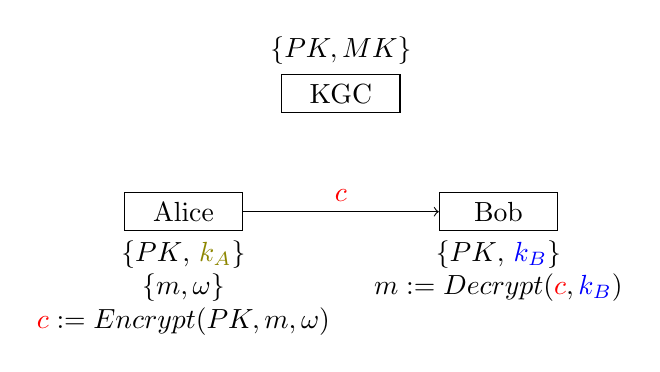
\begin{tikzpicture}[actor/.style={draw, minimum width=1.5cm}]
            \node[actor] (a) at (-2,0) {Alice};
            \node[actor] (b) at (2,0) {Bob};
            \node[actor] (kgc) at (0,1.5) {KGC};
        
            \node[above, align=center] at (kgc.north) {$\{PK, MK\}$};

            \node[below, align=center] at (a.south) {{\{$PK$, $\textcolor{olive}{k_A}$\}}\\$\{m, \omega\}$\\$\textcolor{red}{c}:=\text{Encrypt}(PK, m, \omega)$};
            \node[below, align=center] at (b.south) {\{$PK$, $\textcolor{blue}{k_B}$\}\\$m:=\text{Decrypt}(\textcolor{red}{c},\textcolor{blue}{k_B})$};
            % \node[below, align=center] at (a.south) {$\{PK, k_{A}\}$\\$\{m, \omega\}$};;
            % \node[below, align=center] at (b.south) {$\{PK, k_{B}\}$\\$m:=\text{Decrypt}(c,k_B)$};

            \draw[->] (a) edge node (c) [above] {$\textcolor{red}{c}$} (b);

            % \draw[->] (c.north) -- ++(0,.2) node [anchor=south] {\small $\omega$};
        \end{tikzpicture}
        \caption{Alice can now use the public parameters $PK$ and $\omega$ to encrypt a message for Bob, which he can decrypt only if his access policy $\textcolor{blue}{S_B}$ is satisfied by $\omega$. Note that the \acrshort{kgc} plays no role in this step}
    \end{subfigure}
    \begin{subfigure}[b]{0.4\textwidth}
        \centering
        \begin{tikzpicture}[matrixstyle/.style={
            matrix of nodes,
            nodes in empty cells,
            column sep      = 0mm,
            row sep         = 2mm,
            draw,
            nodes={
                inner sep=1mm,outer sep=1mm,
                minimum size=5mm,
                anchor=center,
                text centered,
                text width=1cm,
                execute at begin node={\small\setlength{\baselineskip}{1em}} % WTF.. see https://tex.stackexchange.com/questions/223065/how-to-increase-line-spacing-in-tikz-node
            }
        }]
            \matrix (m) [matrixstyle] at (0,0) {
                $PK$ & \node[align=left, text width=3.5cm] {Public Key (same\\for all participants)};\\
                $MK$ & \node[align=left, text width=3.5cm] {Master Secret (known\\only to the \acrshort{kgc})};\\
                $k_A, k_B$ & \node[align=left, text width=3.5cm] {Private\\Decryption Keys};\\
                $S_A, S_B$ & \node[align=left, text width=3.5cm] {Access Structures};\\
                $m$ & \node[align=left, text width=3.5cm] {Plaintext message};\\
                $\omega$ & \node[align=left, text width=3.5cm] {Set of attributes};\\
            };
        \end{tikzpicture}
    \end{subfigure}
    \caption[Interaction of Alice, Bob and KGC in an \acrshort{abes}]{
        Alice wants to send an \acrshort{kp-abe} encrypted message $m$ to Bob. She wants to encrypt the message under a set of attributes $\omega$.
        Both Alice and Bob create a desired \gls{access-policy}, $\textcolor{olive}{S_A}$ and $\textcolor{blue}{S_B}$, respectively.
        Note that the \acrshort{kgc} will only issue a corresponding key if it deems that they should be allowed to obtain a key under the given access policy.

        % \begin{itemize}
        %     \item test
        % %     \item $PK$: Public Key (system parameters, equal for all participants)
        % %     \item $S_A, S_B$: Alice's and Bob's Access policies
        % %     \item $k_A, k_B$: Alice's and Bob's private keys (corresponding to $S_A$ and $S_B$)
        % %     \item $m$: Plaintext message
        % %     \item $\omega$: Set of attributes
        % \end{itemize}
    }
    \label{fig:abe-system}
\end{figure}